% created on 30/03/2020
% @author : ebazan
\chapter*{Introduction}
\addcontentsline{toc}{chapter}{Introduction}
In this thesis we present the study of low-level primitives of an image such as contours, color, texture and texture color in search of generating general vision algorithms that later can be useful for autonomous navigation of Unmanned Aerial Vehicles (UAVs). Since such primitives allow to characterize objects in images under various conditions, they have widely been used in image segmentation and modeling tasks. To go further, we take interest in the study of these primitives in combination with some concepts of human visual perception, seeking to achieve high-level tasks such as the scene understanding. For this purpose, we favor traditional Computer Vision (CV) methods, avoiding dependence on finely adjusted parameters, to obtain image features with physical sense that can be used later in completely unsupervised algorithms.

%\section*{Relationship between drones and computer vision }
\section*{Background and Motivation}

The advancement of computer vision techniques has favored its use in a wide range of applications. The development has been outstanding in already traditional application areas such as multimedia or medicine. However, new areas of application such as augmented reality, automated driving, robotics, the Internet of Things (IoT) and the Industry 4.0, human-computer interaction and vision for the blind, continue to emerge . 

Regardless of the application, computer vision systems must perform a number of tasks to achieve their goal. Generally, these tasks include techniques for acquiring, processing, analyzing, and understanding digital images; extracting real-world data to produce symbolic information, for example, in the form of decisions. Depending on the context, understanding images can mean transforming visual images (the sensor input) into descriptions of the world that can interact with other processes and provoke appropriate actions. This compression can be seen as the crumbling of the symbolic information in the image using geometric, physical, statistical or theory of learning models.

More particularly, the tasks of computer vision can be grouped into four more or less well-defined processing problems.

\begin{enumerate}[label=\roman*]
	\item \textbf{Recognition}, a classic problem of computer vision which is responsible for determining whether an image contains any object, characteristic or exercise. Some variants of this problem are the classification, identification and detection of objects from which many specialized tasks emerge. For example, content-based image search, pose estimation, optical character recognition, reading of 2-d codes, facial recognition, shape recognition, among others.
	\item \textbf{Motion analysis}, in which a sequence of images is processed to produce an estimate of the speed of one or more points of interest within a 3-d image or scene. Some examples of this task are egomotion, object tracking, and optical flow.
	\item \textbf{Scene reconstruction}, which is a task related to the computation of a 3-d model from one or more images of a scene.
	\item \textbf{Image restoration}, whose objective is to remove those imperfections of an image generated by disturbances such as sensor noise or motion blur. Generally this task done in the pre-processing stage of the image, before passing it to a more complex algorithm. An example in which this task is applied is inpainting.
\end{enumerate}

While computer vision has outstripped the capabilities of human vision, computers have not completely replaced human personnel. For example, in the case of industrial vision systems tasks, say inspecting bottles or circuit boards on a production line, CV algorithms surpasses humans. However, in areas such as medical imaging, computer vision systems are only responsible for supplementing certain routine diagnoses that require a lot of time and experience from human doctors. This is largely related to the complexity of the task and the conditions under which the application is carried out. In the case of machine vision systems, working conditions are generally controlled, while in areas such as medicine, each patient image is different despite the fact that the acquisition system is the same. Analogously, we can see a similar effect in other areas such as robotics but in particular with unmanned aircraft.

Unmanned aerial vehicles (UAVs) or drones are these flying engines that are increasingly present in our lives. We can found them in various sectors, such as the military, commercial or civil, where they are able to carry out specific tasks quite efficiently. However, in most cases the development of such applications requires an expert pilot to control the aircraft. Commonly, the UAV  control is achieved with the use of conventional sensors, such as inertial sensors (IMUs) for orientation, and GPS for position. The combination of information from these sensors in a flight computer allow the drones to remain stable in the air. The drawback with the IMU is that suffers from bias error propagation due to the integral drift, while with the GPS signal is not always guaranteed. For example, in urban or indoor environments, the satellite signal is low or unexisting. 

A recurrent technique to enhance the position accuracy implies the data fusion of pressure, ultrasonic, radars and laser range-finders sensors \citep{Tomic.Schmid.ea:IRAM:2012}. The fusion of data can provide the advantages of each sensor. However, a major limitation of these complex systems is the flight time, parameter which is mainly linked to the total weight of the vehicle and the capacity of the battery. Therefore, the use of multiple sensors on board becomes expensive and impractical.

It is possible to extend the capabilities of a drone by integrating some type of visual sensor. Contrariwise to other sensors such as Lidars, visual sensors are passive, lightweight and can acquire valuable information about the surrounding structures, including color and textures, and UAV's self-motion. The addition of visual sensors to perceive the environment has been a recurring strategy that has made these aerial robots more manipulable, safer and even in some cases autonomous, that is, that the drone is capable of performing a task without the need for a human intervention. For this, the drone must be able to move without getting lost, but above all, it must be able to detect and avoid potential obstacles on its way. 
Today, one can use different visual sensors; such as monocular cameras \citep{Padhy.Xia.ea:TSC:2018}, stereo cameras \citep{Seitz.Curless.ea:CVPR:2006}, RGB-D cameras \citep{Huang.Bachrach.ea:RobR:2017}, fish-eye cameras \citep{Hrabar.Sukhatme:IROS:2004}, thermal cameras \citep{Gaszczak.Breckon.ea:IRCV:2011}, among others. This wide range of sensors offers more options and flexibility to deal with the problems mentioned above. The integration of such sensors in UAVs has allowed us to see the world from another perspective (literally); and the development of perceptual computer vision algorithms drive the technological development of these machines.

\section*{Problem Statement}
%\section*{Computer Vision Problems in Drone Applications}
 
We can interpret the applications and taks made with drones as missions. Generally, such missions involve three main moments: take-off, navigation, and landing. Although such stages can be done with conventional sensors as mentioned above, the use of visual sensors provides valuable information about the environment. 

Among the three moments that occur in drone missions, navigation and landing are the stages in which visual information from on-board sensors and computer vision algorithms most frequently intervene. In the case of the landing stage, the needs and problems can be well-defined since it occurs at the end of the mission. In addition, we can control some conditions by adding pre-designed elements, for example landing targets or landing platforms, to help in the task. However, in the case of the navigation stage the computer vision problems are mainly determined by the nature of the drone applications. 

Drone missions are generally carried out in complex scenes that change as the vehicle moves through space. For example, imagine all the scenarios that a delivery drone goes through during its mission: It can start its route in a commercial area, where the scenes are mostly cluttered of halls and big open spaces such as parkings. Then, it could pass through rural areas, where the scenes can contain framlands or wooded areas. Finally, when the drone reaches the delivery point within an urban zone, the environment may contain houses, trees, electricity and telecommunications poles, etc. This results in overexposed and/or dark images due to considerable lighting changes and the precense of shadows. In addition to the lack of control of these conditions, we must also consider that the position and orientation of the camera with respect to the scene varies depending on the height and orientation of the vehicle. Therefore, the objects present in the images may have deformations. The figure \ref{fig:img_drone_degradations} shows some images taken with a commercial drone in a real setting. We can observe how the lighting conditions of the environment and the nature of the aerial applications introduce deformations to the images and objects present in the scene. Finally, we must not forget that image acquisition is carried out by an on-board camera, which is generally not stabilized, in consequence, the images may be noisy or blurry. Such problems prevent the existence of any global computer vision algorithm that is efficient in all or most of the situations. 


\begin{figure}[!ht]
    \centering
    \begin{subfigure}[b]{0.38\textwidth}
        \frame{\includegraphics[width=\textwidth]{Bebop_A}}
        \caption{Precence of shadows}
    \end{subfigure}
        ~ %add desired spacing between images, e. g. ~, \quad, \qquad, \hfill etc. 
      %(or a blank line to force the subfigure onto a new line)
    \begin{subfigure}[b]{0.38\textwidth}
        \frame{\includegraphics[width=\textwidth]{Bebop_B}}
        \caption{Saturations}
    \end{subfigure}
        ~ %add desired spacing between images, e. g. ~, \quad, \qquad, \hfill etc. 
      %(or a blank line to force the subfigure onto a new line)
    \begin{subfigure}[b]{0.38\textwidth}
        \frame{\includegraphics[width=\textwidth]{Bebop_C}}
        \caption{Change of scale}
    \end{subfigure} 
    \caption{Some examples of image degradations present in aerial imaging and UAVs applications.}\label{fig:img_drone_degradations}
\end{figure}

In addition to the problems related to the complex scene conditions, we must consider that a drone is subject to sudden changes in the environment, for example wind gusts, which can affect its stability and also modify the visual information of the sensors on board. In such cases, the vison algorithms for drone navigation must be able to process the input information fast enough to provide answers that can be transformed into decision actions in real time.

In the literature we can find a large number of works that deal with drone navigation. Among these works we can say that the different approaches are strongly related and motivated by the aim of the application and the conditions in which it is carried out. However, we can clearly differentiate two main vision-based techniques for UAVs navigation; i) localization and mapping and ii) obstacle avoidance.

The so-called Simultaneous Localization and Mapping (SLAM) falls within the techniques of the first group, where drone navigation is a consistent result. This technique estimates the local pose of a robot and builds a 3-d model of its surroundings employing visual sensors. The Visual Odometry (VO) \citep{Scaramuzza.Fraundorfer:RAM:2011} is responsible of the robot motion estimation while the maps are built with occupancy grid algorithms \citep{Thrun.Bu:AI:1996}. According to the image information used to perform a SLAM, we can classify these approaches into feature-based methods, which extract a set of image features (e.g., lines, points) in a sequence of images, and direct-based methods, which make use of the image intensity information to estimate the structure and the motion of the robot.

The use of SLAM techniques for UAV navigation presents remarkable advantages. Feature-based methods can use a wide variety of feature detectors which counts typically with an optimization stage that allows having fast algorithms. Direct-based methods have the advantage to be robust to images degradations; they can lead better with images with texture and blurred zones; besides, the map produced is of an acceptable resolution. An interesting fact is that the strengths of the first group of methods are the weak points of the second and vice versa. A method that tries to gather the benefits of both approaches is the Semi-direct Visual Odometry \citep{Forster.Pizzoli.ea:ICRA:2014}; however, in general, the SLAM methods works in indoor environments, where the illumination conditions are static or controlled.

On the other hand, there are the approaches for drone navigation that favor the avoidance of obstacles. This capability is of great importance for achieving free collisions missions in both, indoor and outdoor environments. A recurrent solution, as we early mentioned, is the multi-sensor data fusion. \cite{Gageik.Benz.ea:ACCESS:2015} present a platform using low-cost ultrasound and IR sensors; however, despite the obtained results, it utilizes several sensors to recovers environment information and yet, it does not get a perceptual representation of the scene due to the low resolution and perceptive capacity of the sensors. On the other hand, vision-based techniques for obstacle avoidance could identify obstacles and in some cases classify the found object \citep{Li.Ye.ea:IROS:2016}. 

Visual methods for avoidance of obstacles can be classified into two groups. The first, SLAM-based techniques, make use of the principles above. The 3-d reconstruction provides accurate and sophisticated maps and allows the air vehicle to travel with more information about the environment. In \citep{Moreno-Armendariz.Calvo:ICMEAE:2014}, takes this advantage to develop an obstacle avoidance approach for static and dynamic obstacles. 

The second group is the flow-based methods which historically, were inspired by the navigation of insects such as bees \citep{Srinivasan.Gregory:PTBS:1992} or flies \citep{Franceschini.Ruffier.ea:InTech:2009}. Many insects in the wild identify obstacles through the intensity of light. During the flight, their eyes produce an optical flow that provides accurate spatial information. Currently, there are also works inspired by the behavior of the human eye \citep{Al-Kaff.Meng.ea:IVS:2016}. The technique measures the object size from the idea that objects in the robot's field of vision are larger as the obstacle is closer.

The techniques for obstacle detection and avoidance present interesting characteristics and ideas. Notwithstanding, its implementation is strongly linked to an application under certain conditions. In consecuense, Their use would involve a recalibration or readjustment of parameters. Given the conditions in which a drone can operate, it is necessary to have more general and non-supervised methods.

The most efficient algorithms to date are those based on Neural Network (NN) architectures and supervised learning techniques. Nevertheless, these techniques have remarkable disadvantages that question their usability and applicability in real-life drone missions. 
From a practical and even economic point of view, there is a limit to the number of applications in which we can use supervised methods given the fact that we need a lot of annotated data. The collection and the correct labeling of data representative of a problem is true only for a small number of applications. 

The need of abundant information comes with high computational times required for model learning, which can range from a couple of hours to entire weeks. Of course, this variable can be minimized by increasing the computing power of our machines, however, today only those companies that have large computing infrastructures can afford to train models with a thousand of millions of parameters. 
This introduces the next disadvantage of deep neural network based learning models: hyperparameters. Hyperparameters can be roughly divided into two categories, i) optimizer hyperparameters, which include learning rate, batch size, and number of epochs, and; ii) model-specific hyperparameters, including the number of hidden layers, the first hidden layer, and the number of layers. Choosing the appropriate hyperparameters plays a key role in the success of neural network architectures because they control the behavior of the learning algorithm, defining the structure of the network and how the network is trained. Although there are methods to optimize their choice, generally this task is an heuristic process and their fine tuning is a function of the specific application. It is possible to follow some rules based on experience, copy same values from some other problem or make the setting by trial and error, though, we cannot know the best value for a hyperparameter.

\subsection*{Scope of the Thesis}
The interaction between computer vision and applications made with unmanned aerial vehicles is extensive. This collaboration has generated new methodologies and approaches, both theoretical and practical, but has also given way to new research questions. So, we want to detail the scope and focus of this thesis work.

First of all, this thesis work is largely motivated by my profile and interests in the field of robotics and control theory, specifically in air vehicles. Knowing the real limitations of aerial robots and the complexity of applications made with drones, this thesis seeks to explore within the theory of computer vision to propose algorithms that improve and provide assistance in drone navigation task. In this sense, we are interested in the study of the scenes perceptual information for their treatment and interpretation.  

We focus primarily on the first computer vision processing problem of the list mentioned above; recognition. We argue that scene understanding, through object recognition, is a key to UAV navigation, especially in cases where the tasks are developed in complex uncontrolled environments. From this perspective, we focus on the use of low-level image features to extract perceptual information for object detection and segmentation. Throughout this work, we develop vision algorithms that provide solutions to some variants of the recognition problem, such as the classification, identification and detection of objects. 


Throughout this work, we develop algorithms that use such primitives in conjunction with statistical and geometric tools from the area of computer vision and signal theory. The algorithms developed provide solutions to some variants of the recognition problem, such as the classification, identification and detection of objects from a qualitative point of view, always looking for the physical meaning of the application. So it is worth mentioning that the practical aspect linked to the implementation and the generation of solutions in real time are not a priority.

Regarding the nature of the input data, we use only color or black and white images as input information, favoring the use of monocular cameras among the wide range of visual sensors reviewed previously. This provides the possibility of replicating the algorithms with low-cost cameras that can be easily embedded in a drone.

One last point about the focus of this work is about the type of computer vision techniques. The algorithms proposed in this thesis are based on traditional computer vision techniques, that is, non-deep learning techniques. This is consistent with the nature of drone applications, where there are not necessarily rich enough annotated databases to apply the most sophisticated artificial intelligence models.

\section*{Objectives of the Thesis}\label{sec:objectives_of_the_thesis}

In this Ph.D. thesis, we aim to develop general computer vision algorithms with the aim of using them in the frame of UAV navigation. In this context, the primary objective is to propose a new methodological framework for the detection of objects and the understanding of scenes. As we mentioned before, the idea is to apply this framework to provide assistance in control and decision-making in the task of drone navigation. Therefore, the framework must be robust to image degradations existing in environments with uncontrolled conditions, in addition to being independent of the choice of specific parameters for its operation.

During the thesis, many specific drone tasks are considered such as i) environment awareness, ii) detection and avoidance of obstacles, iii) identification and following of targets. Given these tasks, the work focuses on the scene understanding problem. To deal with this problem, we delve into the study of low-level image primitives such as contours, color, texture, and texture color. Therefore, some secondary objectives involve the creation of a representative feature space using concepts from signal theory, geometry and statistics, in addition to concepts from human perception.

The idea is to gather these features under an unsupervised framework and without the need of specific parameters, using traditional machine learning and segmentation algorithms. The figure \ref{fig:general_diagram_framework} shows a general diagram of the framework we propose. Although the framework itself is an ambitious goal, in this thesis we present several algorithms, which use the framework with one or more features, in solving different problems of computer vision such as object detection and recognition, image retrieval systems, perceptual object boundaries detection and image segmentation.

The interest of obtaining a representative space of the image information from low-level hand-made features is that it is possible to use them in a semi-supervised pipeline. By injecting annotated information into the frame, he might be able to make generalizations and obtain medium- or high-level features such as the importance of color and texture information to a human when segmenting an image.

\begin{figure}[!ht]
    \centering
    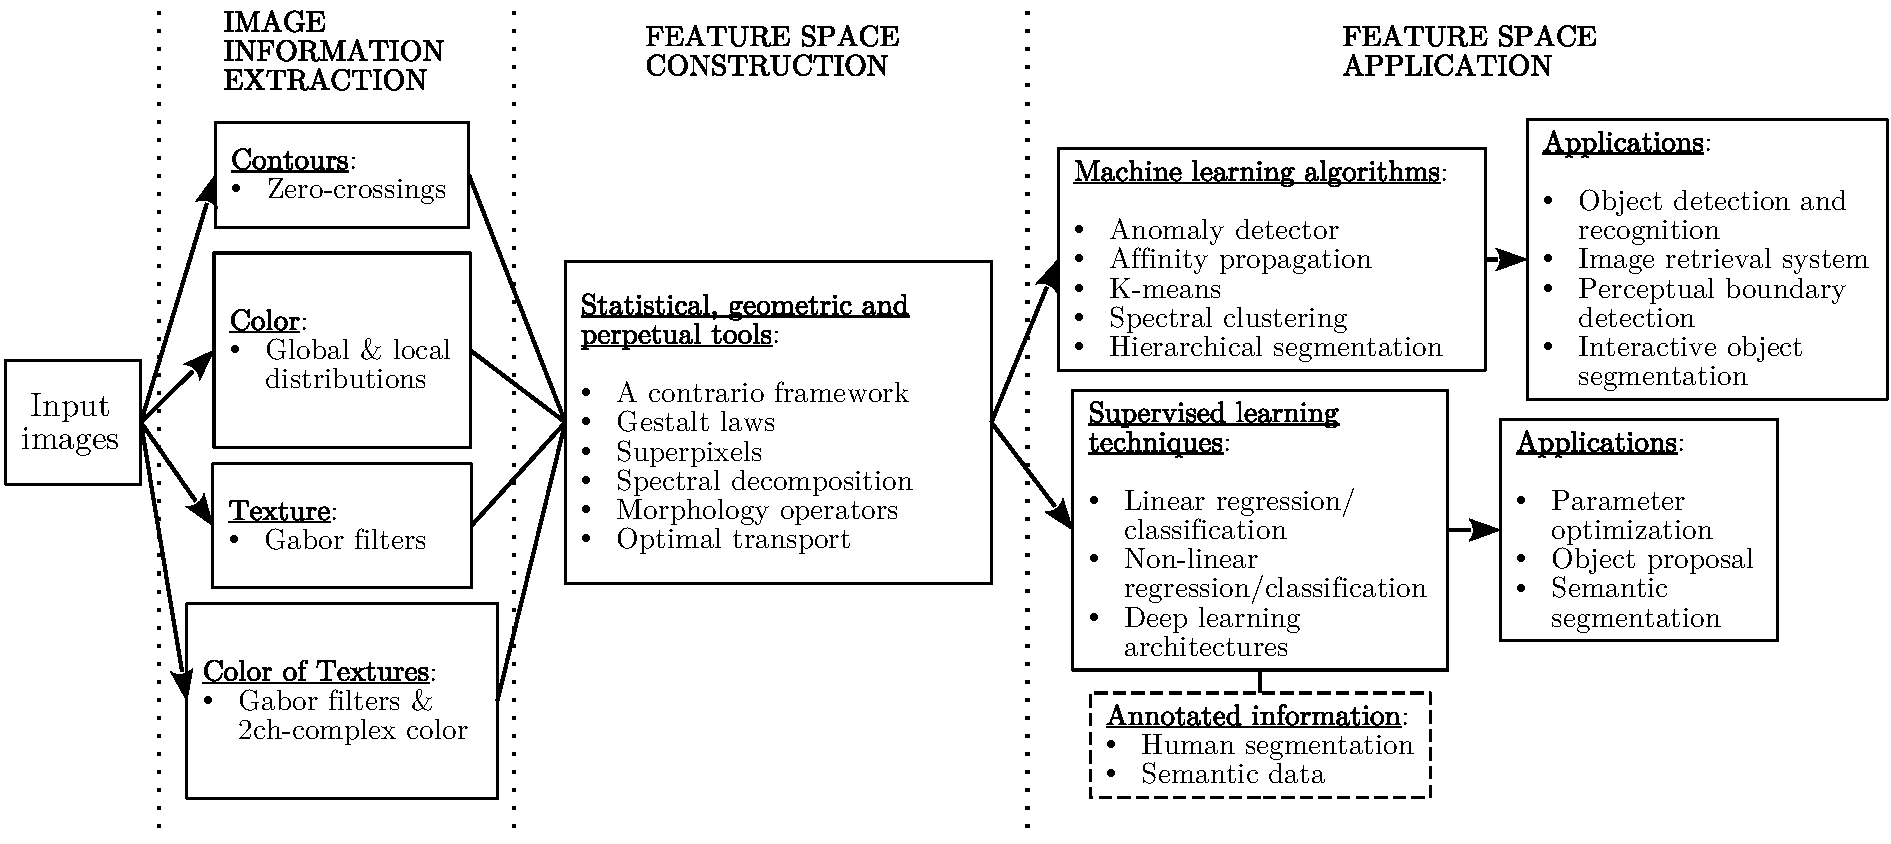
\includegraphics[width=\textwidth]{general_framework_diagram}        
    \caption{Proposed framework for object detection and scene understanding.}\label{fig:general_diagram_framework}
\end{figure}

Throughout the study of each of the low-level primitives and their resulting feautues, several secondary targets are present.

\begin{itemize}
	\item \textbf{Framework implementation.} Referring in a first stage to the implementation in simulated and off-board environments. In a second moment, to the implementation in a real platform. The latter requires the search for a portable platform capable of real-time operation.
 
	\item \textbf{Framework functional evaluation.} Comparison of the obtained results with respect to the approaches of state of the art.
 
 	\item \textbf{Framework validation.} Real test deployment taking into account the constraints of portability and real-time on the industrial scale.
 
\end{itemize}

Finally, this thesis aims to show that traditional computer vision methods are (still) a reliable option to develop the object detection and recognition. Especially in the current context of computer vision, where there are hundreds of algorithms based on neural networks and artificial intelligence for image segmentation and object detection that are highly performant, but lack a physical (and in many cases logical and argued) interpretation of its results. Furthermore, these algorithms are in trouble when it comes to image analysis of complex scenarios or applications where there are no a database rich enough to do the learning process.


\section*{Organization of the Document}
We explore three low-level primitives during this thesis; contours, color and texture. The organization of this document follows to some extent the evolution of the construction of the vision-based framework for object detection and aid in drone navigation. This thesis will then be decomposed into three parts:

\begin{enumerate}
	\item A part dedicated to the study of the contours of the image, in which we review in detail some of the classic methods for obtaining image contours. We use this information in conjunction with the \textit{a contrario} method and the Gestalt organizing laws to perform the detection and identification of landing targets.
	\item The second part is dedicated to the study of the color and texture of an image. In particular, we are interested in the global distribution of this information and the existing metrics to measure the similarity between the distributions. We apply and validate these concepts in a retrival image system.
	\item In the third and last part of this work, we extend the study of color and texture in images, this time we are interested in the local distribution of these primitives. We also study the influence of color information on the creation of textures in an image. We propose a completely unsupervised framework for the detection of perceptual bondaries. Furthermore, we explore different strategies to obtain the segmentation of natural images using the obtained perceptual boundaries.
\end{enumerate}

More specifically, the chapters contained in the three sections are structured as follows:

\begin{itemize}
	\item \textbf{Chapter \ref{ch:landing_target_detection}} addresses the problem of autonomous drone landing using computer vision. We present an algorithm for the detection of landing targets under an unsupervised frame based on the perceptual contours of an image. The chapter is a reminder of different traditional methods for the extraction of contours and some concepts of human perception such as the Helmholtz principle and the laws of Gestalt. 
	
	\item \textbf{Chapter \ref{ch:color_texure_representations}} presents a detailed review of the different ways to represent the color and texture information in an image. The chapter contains a review of the various color spaces and their main properties, as well as an introduction to the different techniques for characterizing textures in the literature. Such information is of relevant importance in the construction of the framework and the approaches to measure similarity between distributions.
	
	\item \textbf{Chapter \ref{ch:similarity_measures}} presents the analysis between different measures of similarity between distributions, showing the advantages and disadvantages of each of them. In particular we focus on the theory of optimal transport through the Earth Mover's Distance. We show the advantages of this metric over traditional similarity measures using an image retrieval system based on the global color and texture information of an image.
	
	\item \textbf{Chapter \ref{ch:spectral_image_decomposition}} delves into the physical and human perception aspects of Gabor's filters. We show the steps involved in designing an optimized and efficient Gabor family of filters. The proposed filter family models and captures the texture information through an energy efficient decomposition of the image. Such spectral decomposition of the image deals with the Heisneberg’s uncertainty principle. The chapter presents the description of parameters that allow a complete customization of the filter set according to the application.
	
	\item \textbf{Chapter \ref{ch:complex_spectral_image_decomposition}} brings an analysis of the texture information present in color images, showing the strong relationship between those two features. Using the spectral analysis of an image with the previously defined Gabor filters, we generate a feature space that captures the color and texture information simultaneously. We show the richness of such feature space by performing unsupervised image segmentation only using simple clustering techniques.
	
	\item \textbf{Chapter \ref{ch:perceptual_object_boundaries_detection}} introduces a framework for the detection of perceptual boundaries of objects present in natural images. This framework brings together the concepts addressed throughout this document such as the spectral decomposition of the image, the optimal transport as a true metric, and the relationship between color and texture information. In addition, using the hierarchical segmentation technique, we segment natural images in an unsupervised manner. We perform a quantitative and qualitative validation of our method using a known database.
	
	\item \textbf{Chapter \ref{ch:general_discussion}} is dedicated to the discussion of the different results presented throughout this manuscript.
	
	\item \textbf{Chapter \ref{ch:general_conclusions}} contains the general conclusions of the thesis in addition to addressing the different possible lines of research as a continuation of this work.
	
\end{itemize}